\documentclass[../main.tex]{subfiles}
\begin{document}
\chapter{Summary and conclusions}\label{chapter6}
We constructed a sequence of fully consistent static expanded envelopes and winds resulting from near or super-Eddington luminosities in X-ray bursts. We considered a neutron star with a mass of $1.4M_\odot$ and radius of $12$ km, and pure helium composition. These and other parameters relating to the base and photospheric boundary conditions can easily be changed to calculate new models, with the codes made publicly available on \textit{Github}\footnote{\url{https://github.com/simonguichandut/GR-wind}\\\hspace*{0.6cm}\url{https://github.com/simonguichandut/GR-envelope}}. 

For winds (Chapter \ref{chapter3}), we found that high mass-loss rate models were bound to reach a limit where the solution is radiation pressure dominated at the base. For our parameters, this happened at $\Mdot\gtrsim 10^{18.5}$ g s$^{-1}$. We rejected these models because they could not be properly matched to the static burning layer. The remaining models still cover a wide range of base luminosities redshifted to infinity, of ${\sim}\Ledd$ to ${\sim}2.5\Ledd$. In all cases, the excess luminosity is completely transferred to the gas in order to accelerate it and escape the gravitational attraction of the star, such that every model is only slightly super-Eddington at the photosphere. This is in line with what is usually assumed by observers for PRE bursts.
We found that the photospheric radii of these wind models was always large (over 100 km), even for neutron stars with different masses and radii. According to this, the bursts from 4U 1820-30 presented by \citet{Strohmayer2019} and discussed in Chapter \ref{chapter1} had PRE phases driven static envelopes and not winds. It would be interesting to verify if this result holds in multi-dimensional calculations, since factors such as rotation and ignition asymmetry could make the photospheric radius dependent on angle. We also looked at spectral shift and determined that, although small, blueshifts from wind velocities could completely counteract gravitational redshift at large radii, making the total shift of the line nearly zero. We do not expect spectral shifts larger than 1\%, which cannot reproduce the relative line shift result of over 4\% in \citet{Strohmayer2019}. A possible explanation is that absorption and emission lines are produced earlier than the continuum photosphere, something that can only be properly accounted for by models with detailed, frequency-dependent radiative transfer. 
%We found the velocity at infinity to always be less than 1\% of the speed of light. This casts some doubt into the recent suggestion that blueshift from gas velocities could cause spectral shifts  of emission and absorption lines, suggesting that the main factor of such shifts is gravitational redshift. 

For envelopes (Chapter \ref{chapter4}), we found that the luminosity was only slightly sub-critical in the extended region of every model, indicating a fragile balance between gravity and radiation pressure for these envelopes to remain static. This could be related to the fact that these regions are nearly convective. We found that very extended models, with photospheric radii of ${\sim}100-1000$ km, have slightly super-Eddington luminosities, showing that these luminosities do not automatically imply outflows. Lastly, we showed that the method of using the PRE touchdown radius to infer the neutron star radius was prone to errors of hundreds of meters or more if the luminosity is large enough at touchdown and an expanded envelope is still present. 

In comparing the two radius expansion regimes (Chapter \ref{chapter5}), it is clear that envelopes and winds are in the same hydrostatic regime near the surface, an expected result for using the same equation of state. However, the transition in the extended zones is discontinuous, which is evident from the photospheric radii profiles in Fig.~\ref{fig:triple}. Thus, the transition from sub to super-Eddington in the burst rise, and vice-versa in the burst decay, cannot be properly modelled quasi-statically, i.e. with stationary solutions; time-dependent calculations are required. However, the timescales for the compact envelopes and the winds are small enough that these models can be used to interpret data during and after the PRE phase of the burst. One clear improvement that could be made is the implementation an optically thick to thin transition in the wind models, as the definition of the photosphere in a pure optically thick model is imprecise. At the moment of writing this thesis, this is something that we are working on and plan to publish in the near future. 

Our takeaway from this work is that these burst expansion regimes, which are to this day relatively unexplored in the literature, still have many aspects that are not well understood, and that there are many caveats in using them to interpret burst observations. There needs to be more work done to improve these models and understand their properties better. The most pressing issue is to do time-dependent, general relativistic simulations of high luminosity bursts in order to understand the transition from static envelopes to winds, and vice-versa. These could then be connected to a stellar evolution code in order to follow the evolving composition of the outflows and predict spectral line effects. This was done by \citet{YuHangWeinberg2018}, but with only one set of burst parameters and without general relativity which is, as it turns out, a crucial aspect of this problem. Then, this problem should eventually be studied with multi-dimensional simulations to see the impact of effects such as rotation, magnetic fields and ignition asymmetry on the observational signature of these bursts. In Table \ref{tab:futurework}, we summarize what constitutes, in our view, the most important improvements that must be made to burst models in order to properly answer questions about photospheric radius expansion, including those discussed in Chapter \ref{chapter1}. These improvements will be the primary focus of my (\textit{the author's}) doctorate research project, set to begin in September 2020.

\begin{table}[h!]
    \centering
    \caption{Future work}
    % \vspace*{1mm}
    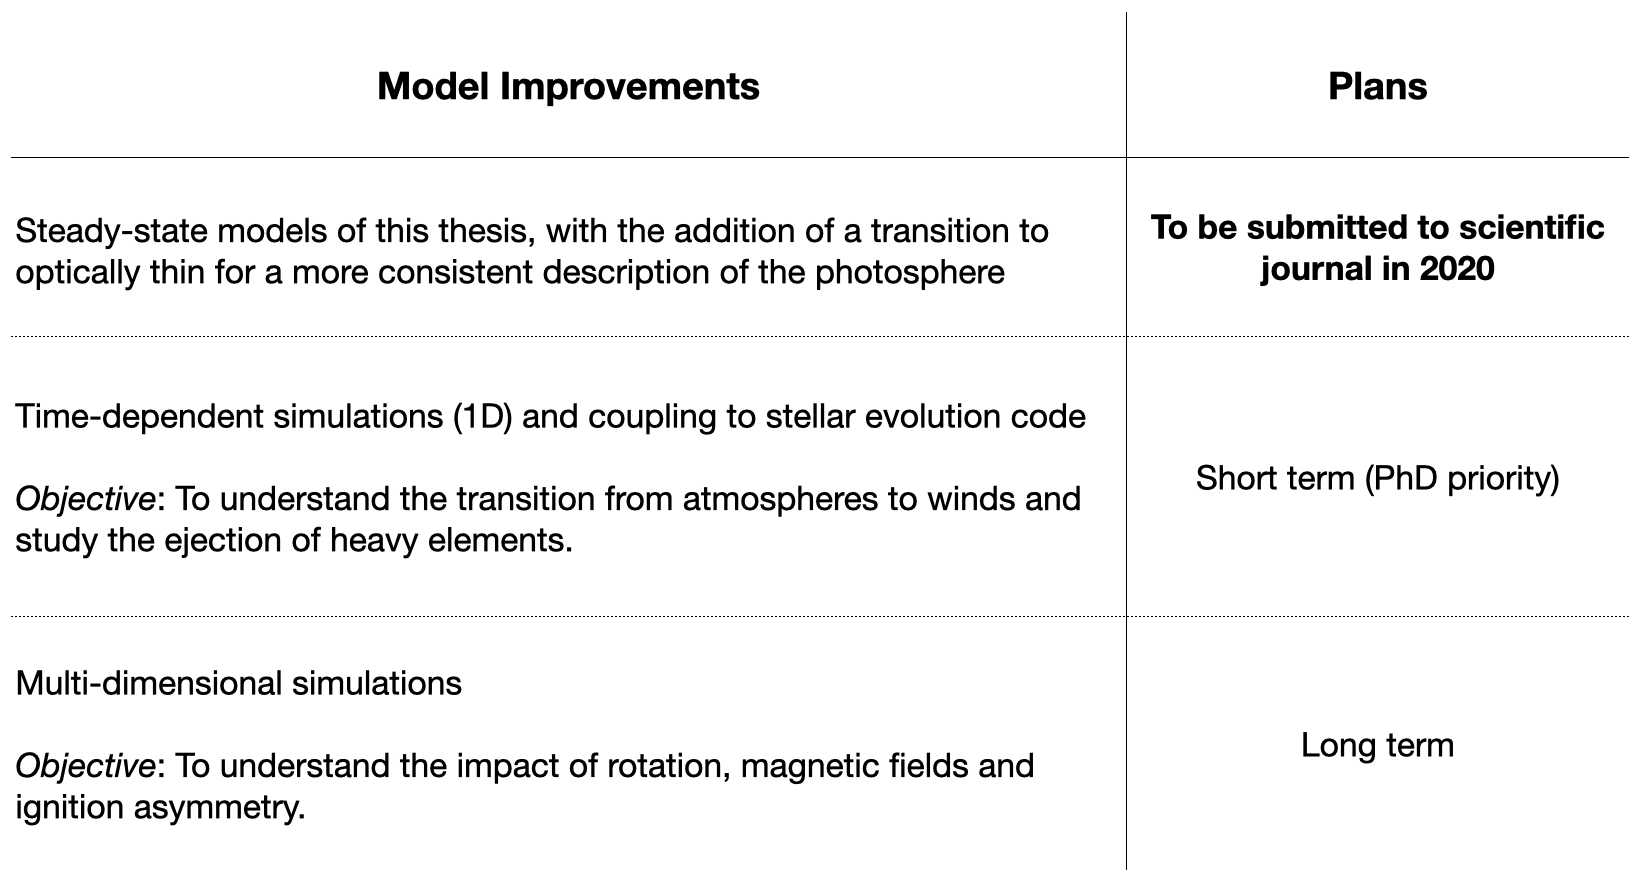
\includegraphics[width=0.9\textwidth]{figures/table2.png}
    \label{tab:futurework}
\end{table}

\newpage

Let us close on the note that the equations for radiation hydrodynamics derived in Chapter \ref{chapter2} (and Appendix \ref{appendix_derivations}), and the numerical methods presented in chapters \ref{chapter3}-\ref{chapter4} can be used to model other astrophysical phenomena in which high luminosities drive stellar outflows. In particular, classical novae are thermonuclear bursts on accreting white dwarfs that result in bright X-ray flashes, very similar to X-ray bursts. Super-Eddington luminosities are attained as well, resulting in mass ejection from optically thick winds \citep{Kato1983}. But in these events, 10 to 90\% of the accreted mass can be ejected \citep{Lewin2006}, much more than in the neutron star case where the strong surface gravity allows no more than ${\sim}$1\% to be unbinded. As a result, classical novae are very different observationally, mainly due to the fact the X-ray flash lasts for months rather than minutes. Nevertheless, the radiation hydrodynamics principles are the same, which should motivate collaboration between theorists in both fields.

\biblio
\end{document}
